
\documentclass{beamer}

\usepackage{algpseudocode, color, colortbl, listings, MnSymbol}

\usepackage{hyperref}
\hypersetup{
    colorlinks=true,
    urlcolor=blue,
}

\usetheme{Montpellier}
\usecolortheme{rose}

% page numbers, from
% https://tex.stackexchange.com/questions/137022/how-to-insert-page-number-in-beamer-navigation-symbols
\expandafter\def\expandafter\insertshorttitle\expandafter{%
  \insertshorttitle\hfill%
  \insertframenumber\,/\,\inserttotalframenumber}

\definecolor{Gray}{gray}{0.8}
\newcolumntype{g}{>{\columncolor{Gray}}c}

\newcommand{\stanza}{ \\~\ }

\title{16. Closest Pair Problem}
\subtitle{CPSC 535}
\author{Kevin A. Wortman}
\institute{ 
\includegraphics[height=2cm]{csuf-logo-cmyk} }
\date{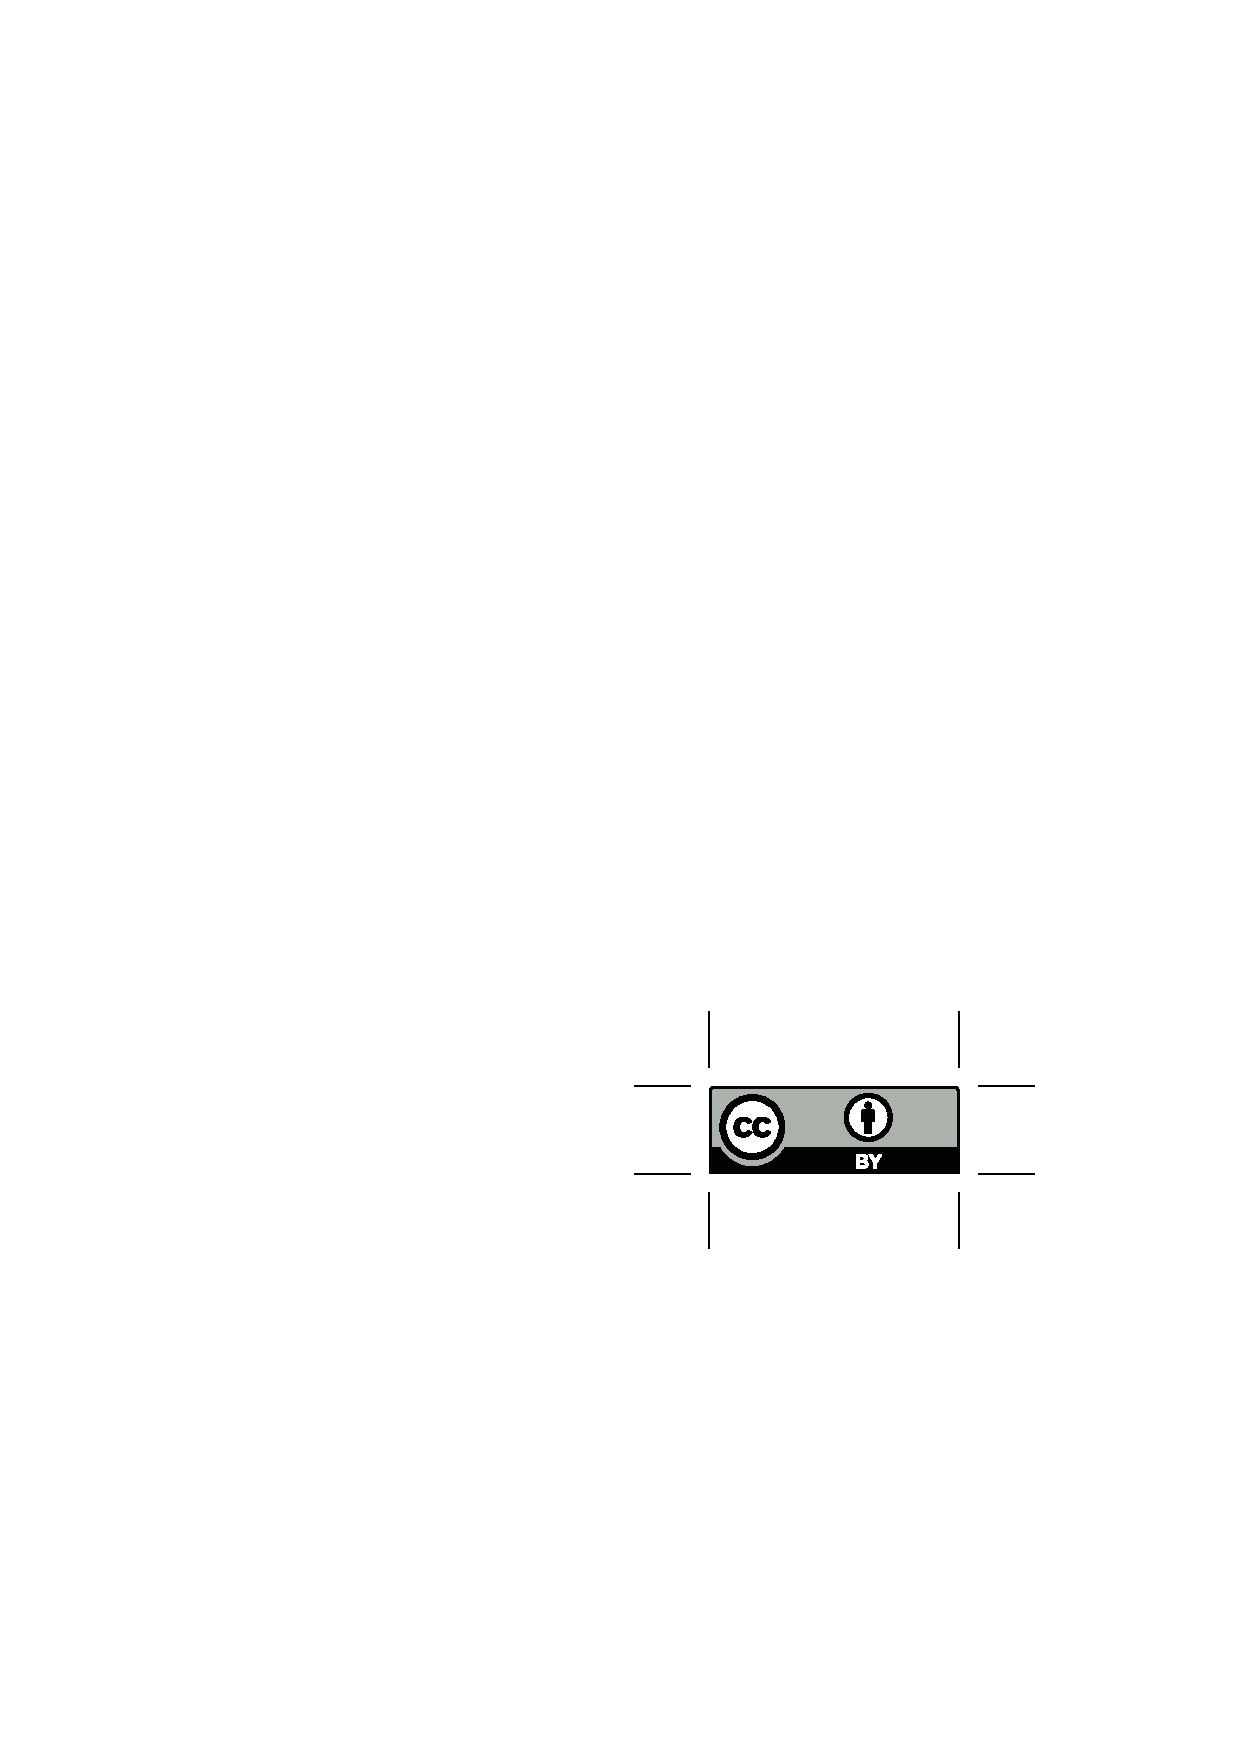
\includegraphics[height=14pt]{by} \\

{\tiny
This work is licensed under a
\href{http://creativecommons.org/licenses/by/4.0/}{Creative Commons Attribution 4.0 International License}.
}}

\begin{document}

\begin{frame}
  \titlepage
\end{frame}

\begin{frame} \frametitle{Closest Pair Problem}
  \emph{closest pair problem} \\
  \textbf{input}: set of $n \geq 2$ planar points $Q$ \\
  \textbf{output}: two points $p, q \in Q$ minimizing $d(p, q)$ \stanza

  $d(p, q)$ is standard Euclidean distance
  \[ d( (x_p, y_p), (x_q, y_q) ) \equiv \sqrt{(x_p-x_q)^2+(y_p-y_q)^2} \]
\end{frame}

\begin{frame} \frametitle{Closest Pair Applications}
  Applications
  \begin{itemize}
    \item find two objects at greatest risk of collision
    \item determine numerical precision needed for points
    \item match predicted user preference to products
    \item match players for fair contest
  \end{itemize}
\end{frame}

\begin{frame} \frametitle{Example}
  \begin{center}
    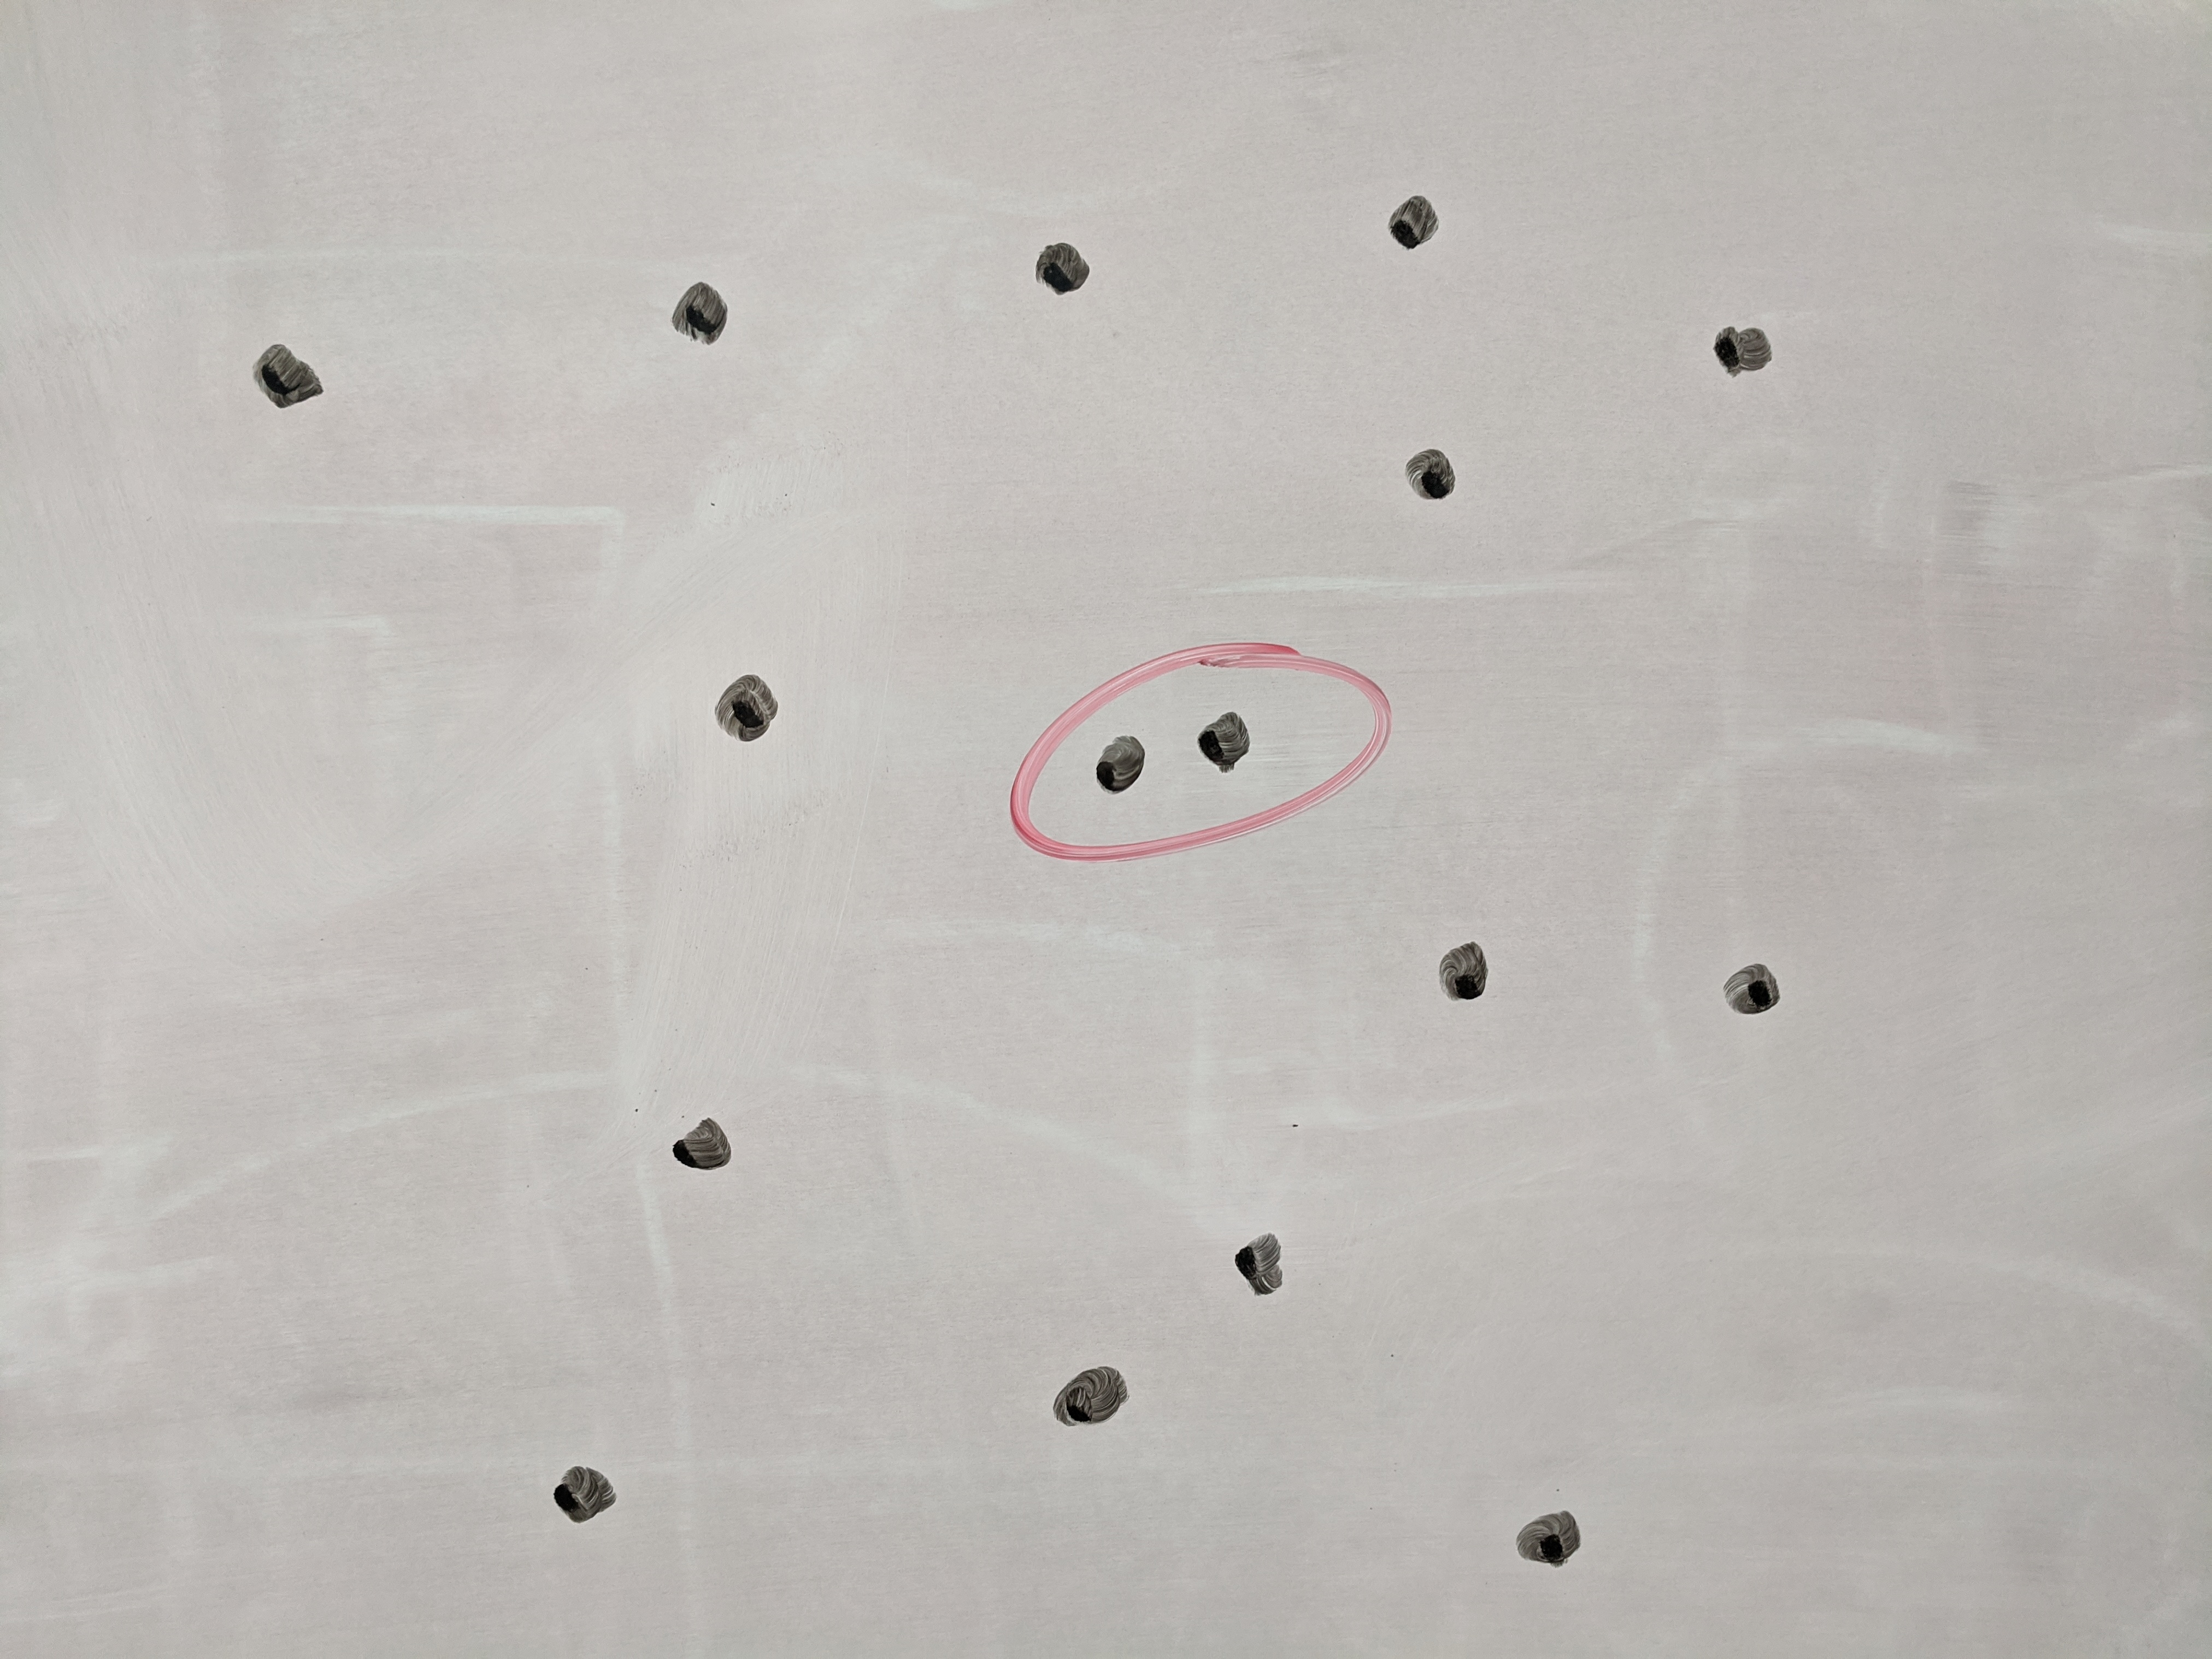
\includegraphics[height=2.5in]{closest-pair-example.jpg}
  \end{center}
\end{frame}

\begin{frame} \frametitle{Baseline Algorithm}
  {\small
\begin{algorithmic}[1]
  \Function{CLOSEST-PAIR-NAIVE}{$Q$} \Comment{guaranteed $|Q| \geq 2$}
    \State $p = q = NIL$
    \State $\delta = \infty$
    \For { distinct $a, b \in Q$ }
      \State $\delta_{ab} = d(a, b)$
      \If { $\delta_{ab} < \delta$ }
        \State $p=a, \, q=b, \, \delta=\delta_{ab}$
      \EndIf
    \EndFor
    \State \Return $p, q$
  \EndFunction
\end{algorithmic}
}

\textbf{Analysis}: $\Theta(n^2)$
\end{frame}

\begin{frame} \frametitle{Divide-and-Conquer First Draft}
\begin{itemize}
  \item base case: $n \leq 3,$ use baseline algorithm
  \item else draw vertical line $\ell$ dividing $Q$ into halves $L, R$
  \item recursively find closest pairs $p_L, q_L$ and $p_R, q_R$
  \item solution is one of
  \begin{itemize}
    \item (from the left) $p_L, q_L$
    \item (from the right) $p_R, q_R$
    \item (straddling the boundary) some $p \in L$ and $q \in R$ even closer
      than $d(p_L, q_L)$ and $d(p_R, q_R)$
  \end{itemize}
  \item na\"{i}ve search for straddling case is $\Theta(n^2) \implies$ need to
    be more clever to speed up
  \item clever $=$ use geometry
\end{itemize}
\end{frame}

\begin{frame} \frametitle{Divide-and-Conquer: Closest Pair on the Left}
  \begin{center}
    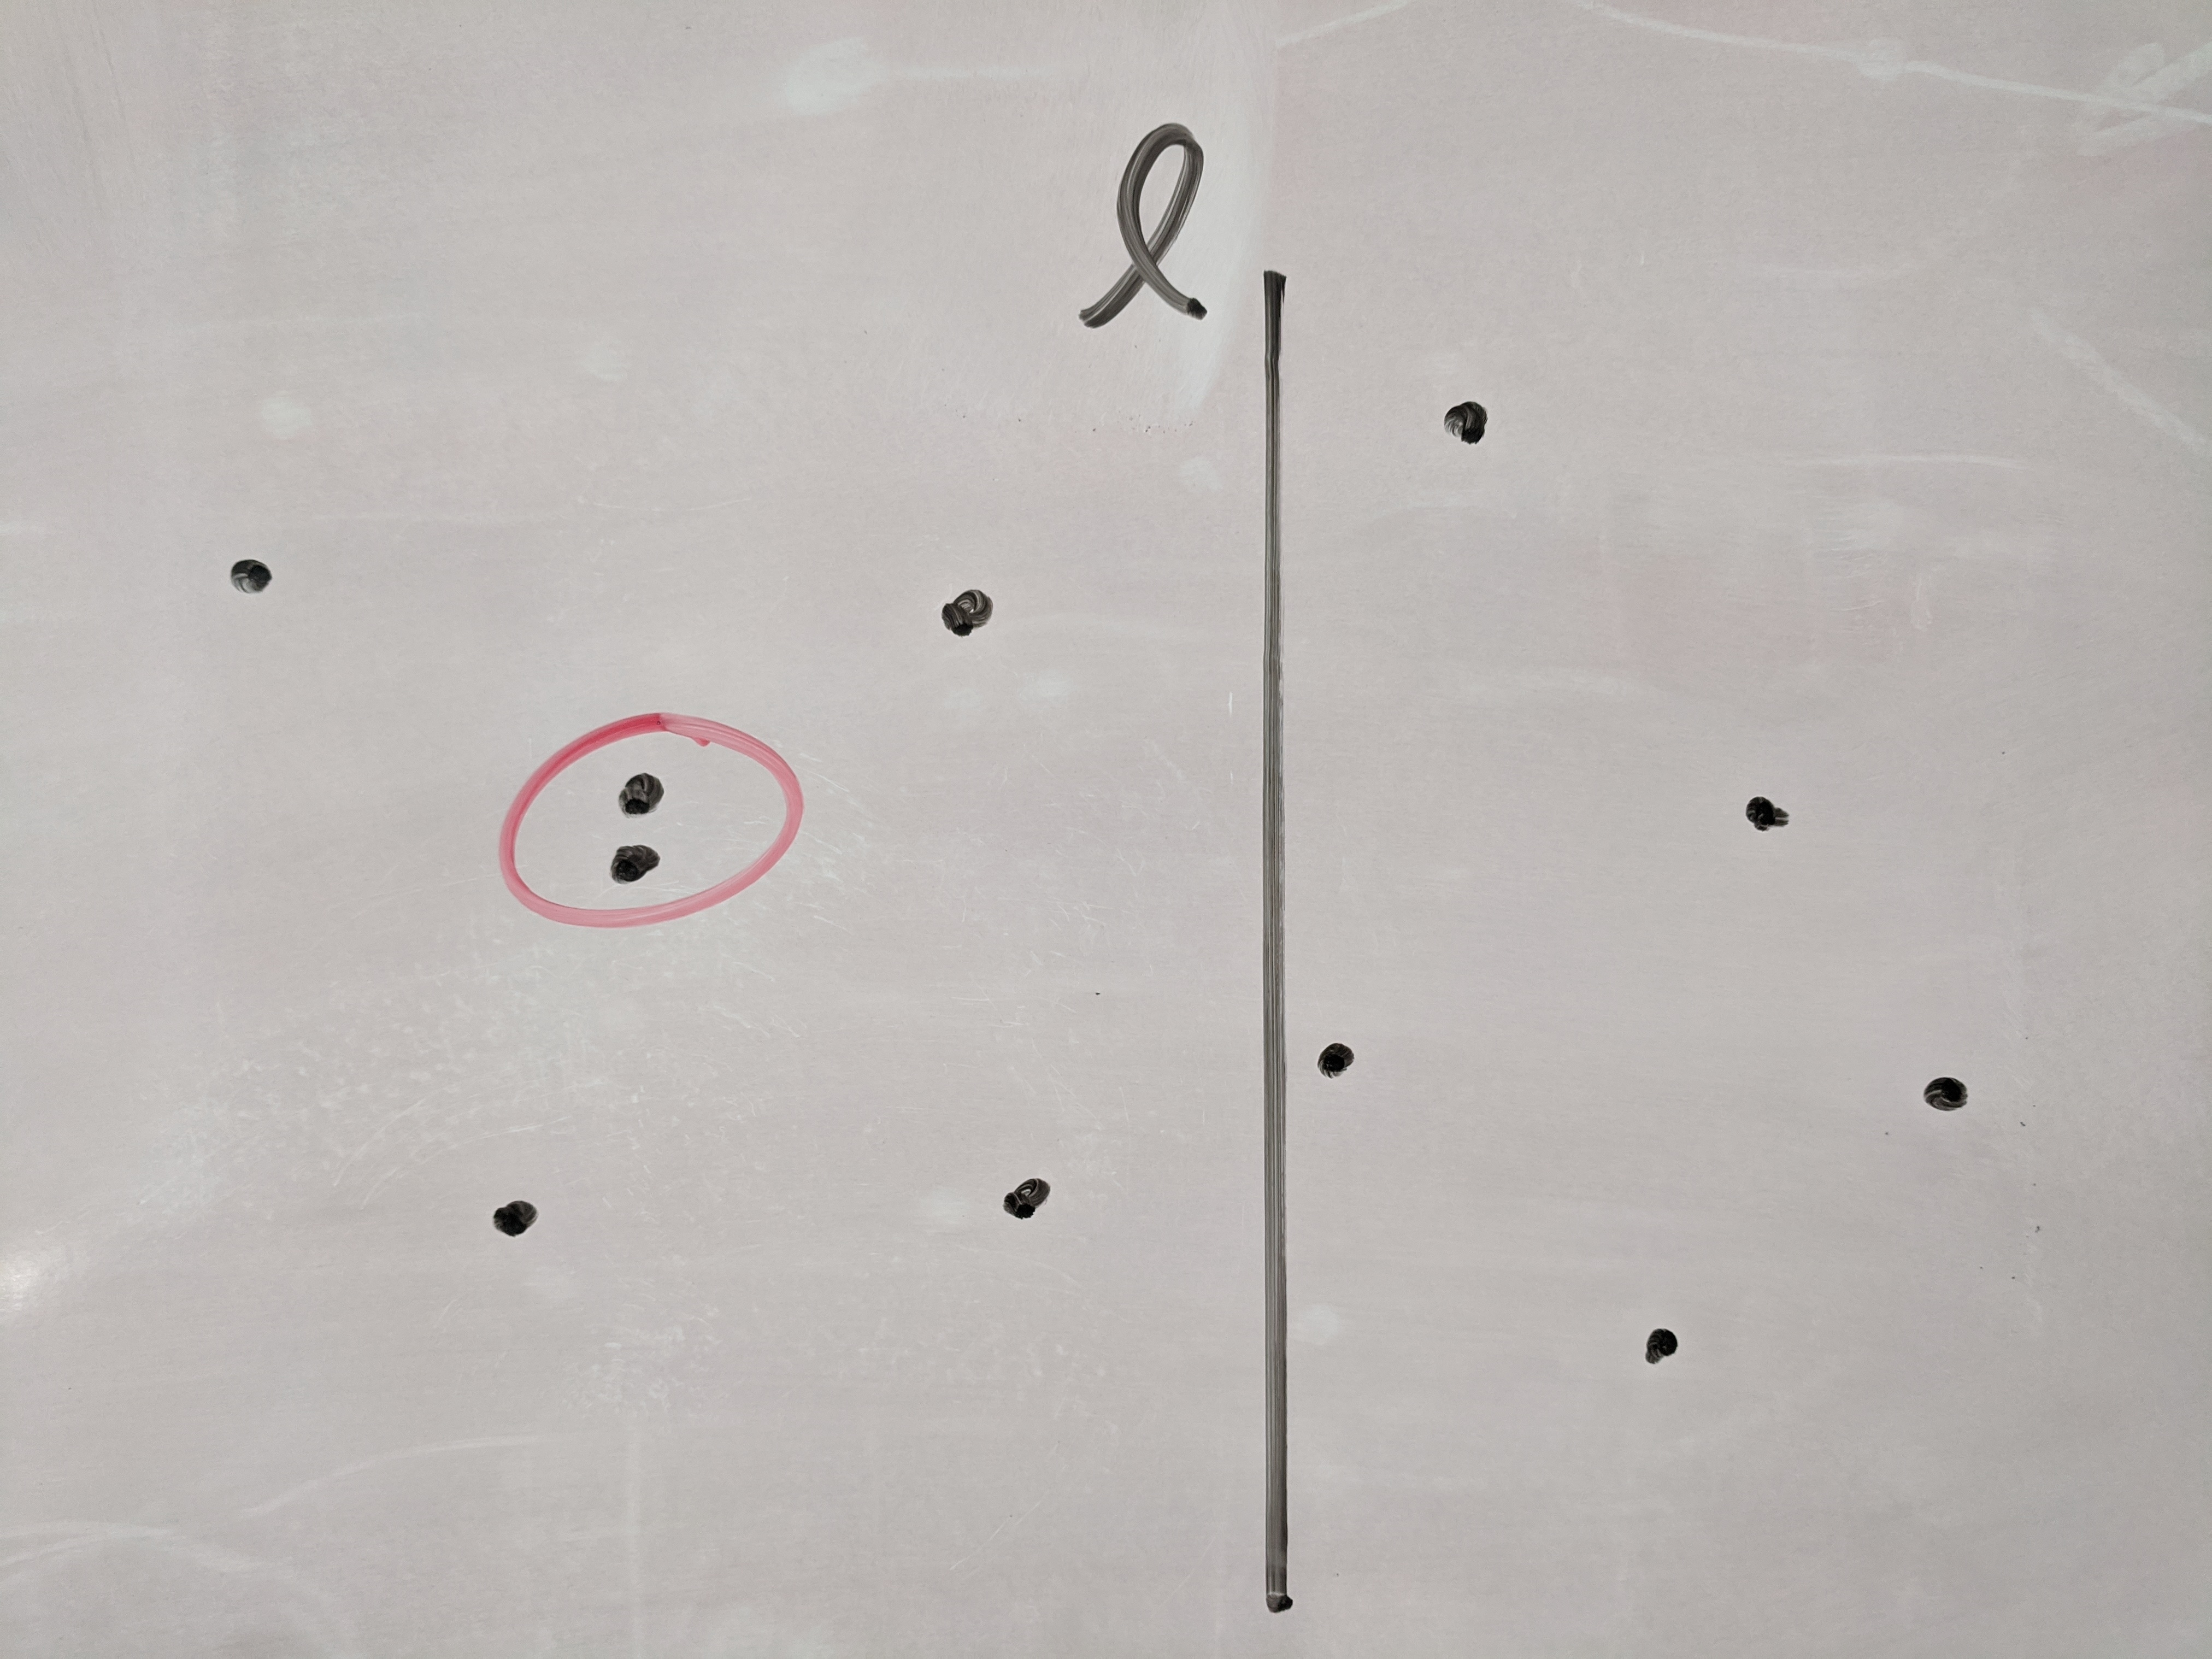
\includegraphics[height=2.5in]{closest-pair-on-left.jpg}
  \end{center}
\end{frame}

\begin{frame} \frametitle{Divide-and-Conquer: Closest Pair on the Right}
  \begin{center}
    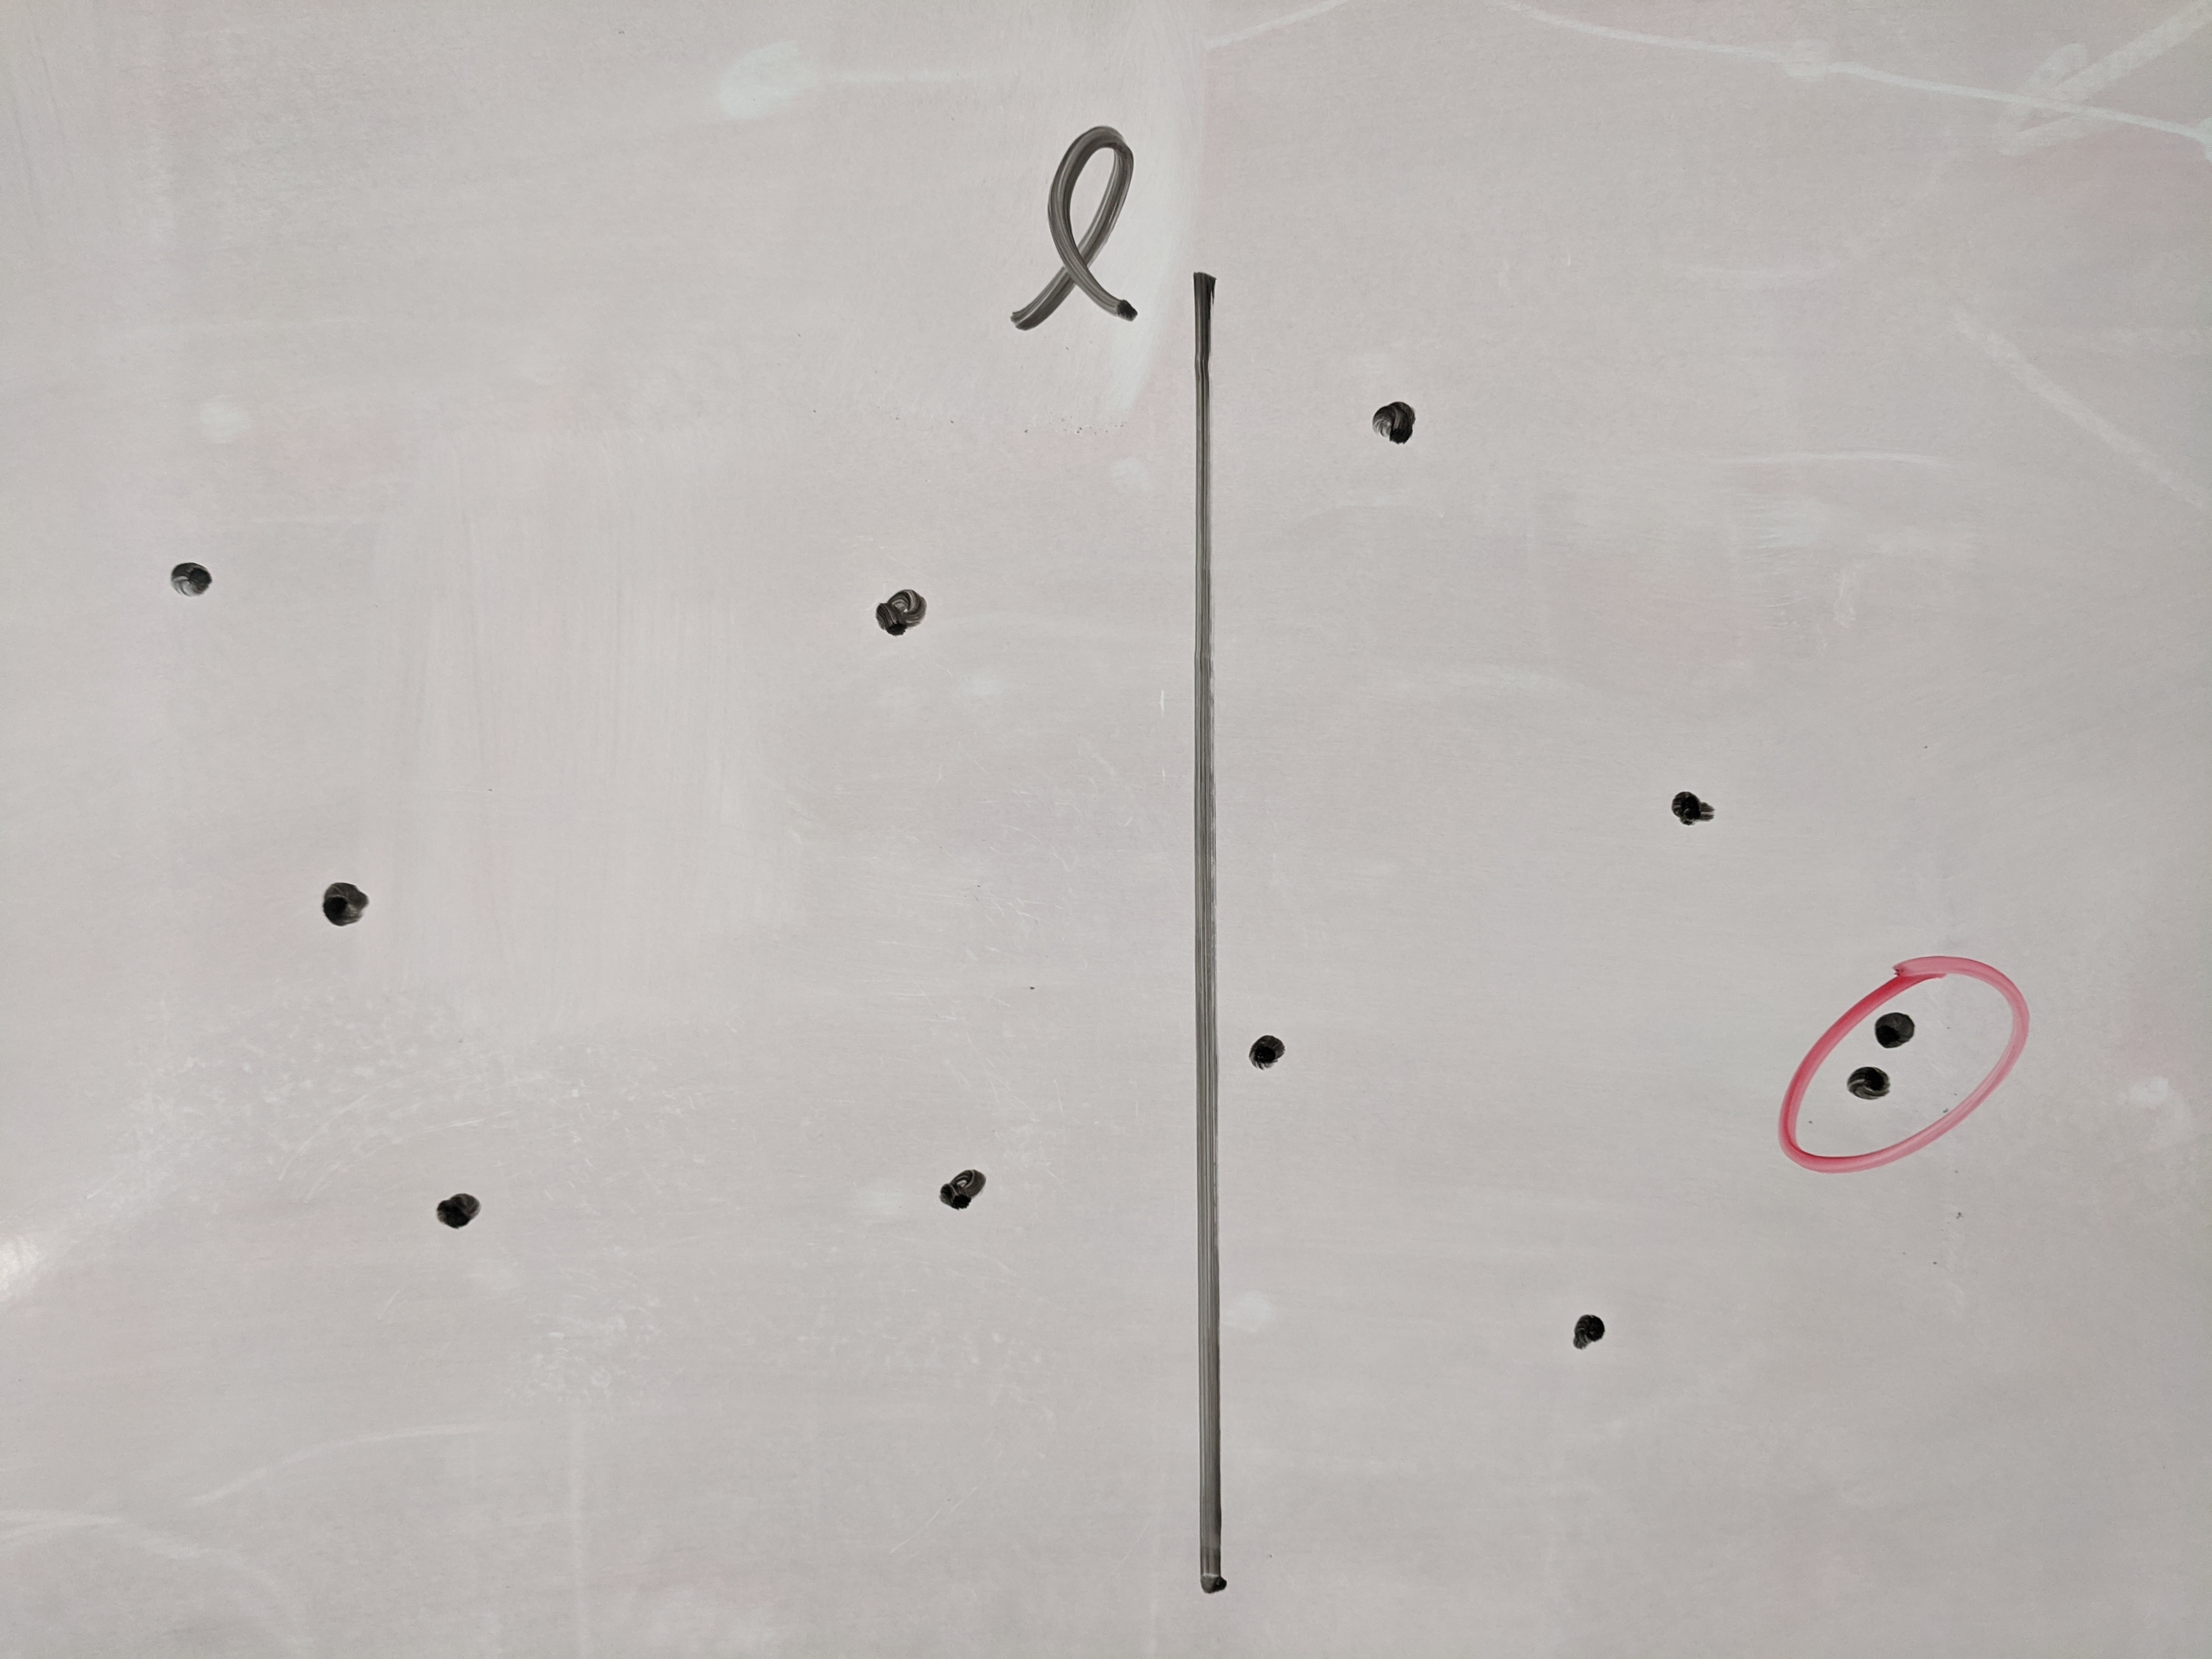
\includegraphics[height=2.5in]{closest-pair-on-right.jpg}
  \end{center}
\end{frame}

\begin{frame} \frametitle{Divide-and-Conquer: Closest Pair on the Boundary}
  \begin{center}
    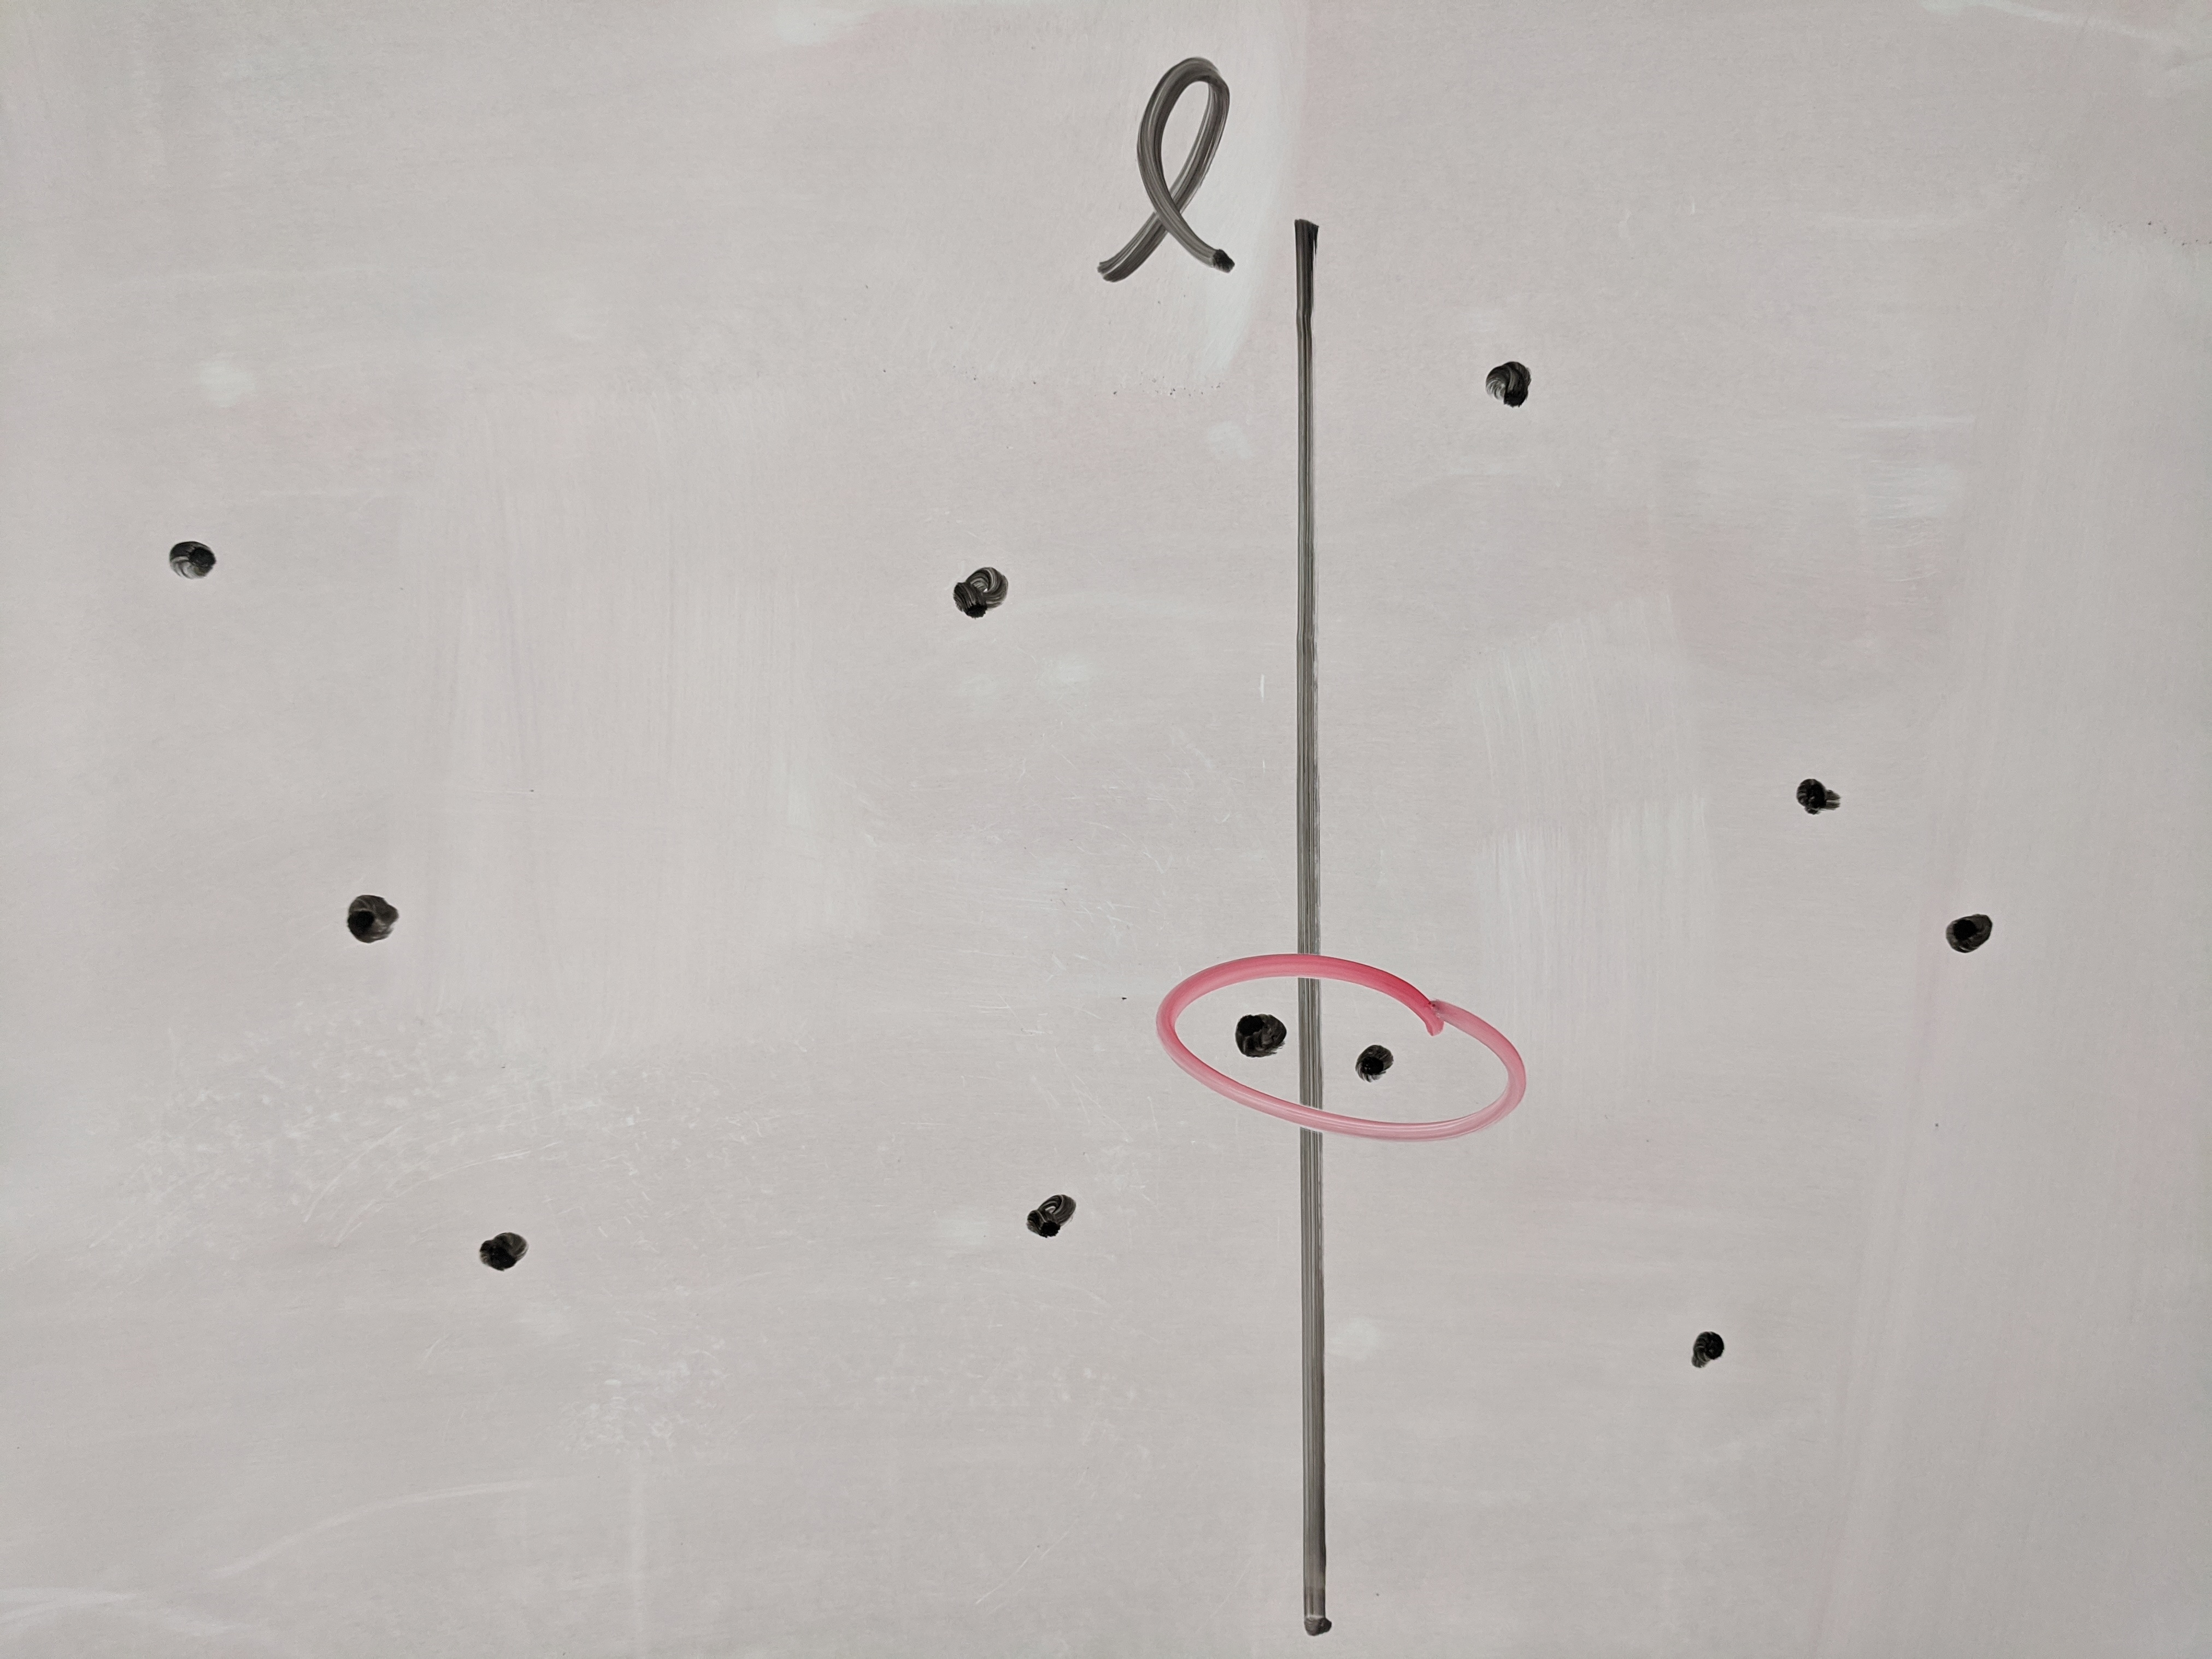
\includegraphics[height=2.5in]{closest-pair-on-boundary.jpg}
  \end{center}
\end{frame}

\begin{frame} \frametitle{Narrowing Search at Boundary}
\begin{itemize}
  \item \textbf{Claim}: only need to check $O(n)$ pairs of straddling points, not $\Theta(n^2)$
  \item let $\delta = \min(d(p_L, q_L), d(p_R, q_R)) = $ distance between closest
    pair entirely in $L$ or entirely in $R$
  \item suppose $\exists p_S$ left of $\ell,$ $q_S$ right of $\ell,$ with $p_S, q_S$ closer than $\delta$
  \item such $p_S, q_S$ must reside in a $2\delta \times \delta$ rectangle centered on $\ell$
\end{itemize}
\end{frame}

\begin{frame} \frametitle{Region that Could Contain a Closest Straddling Pair}
  \begin{center}
    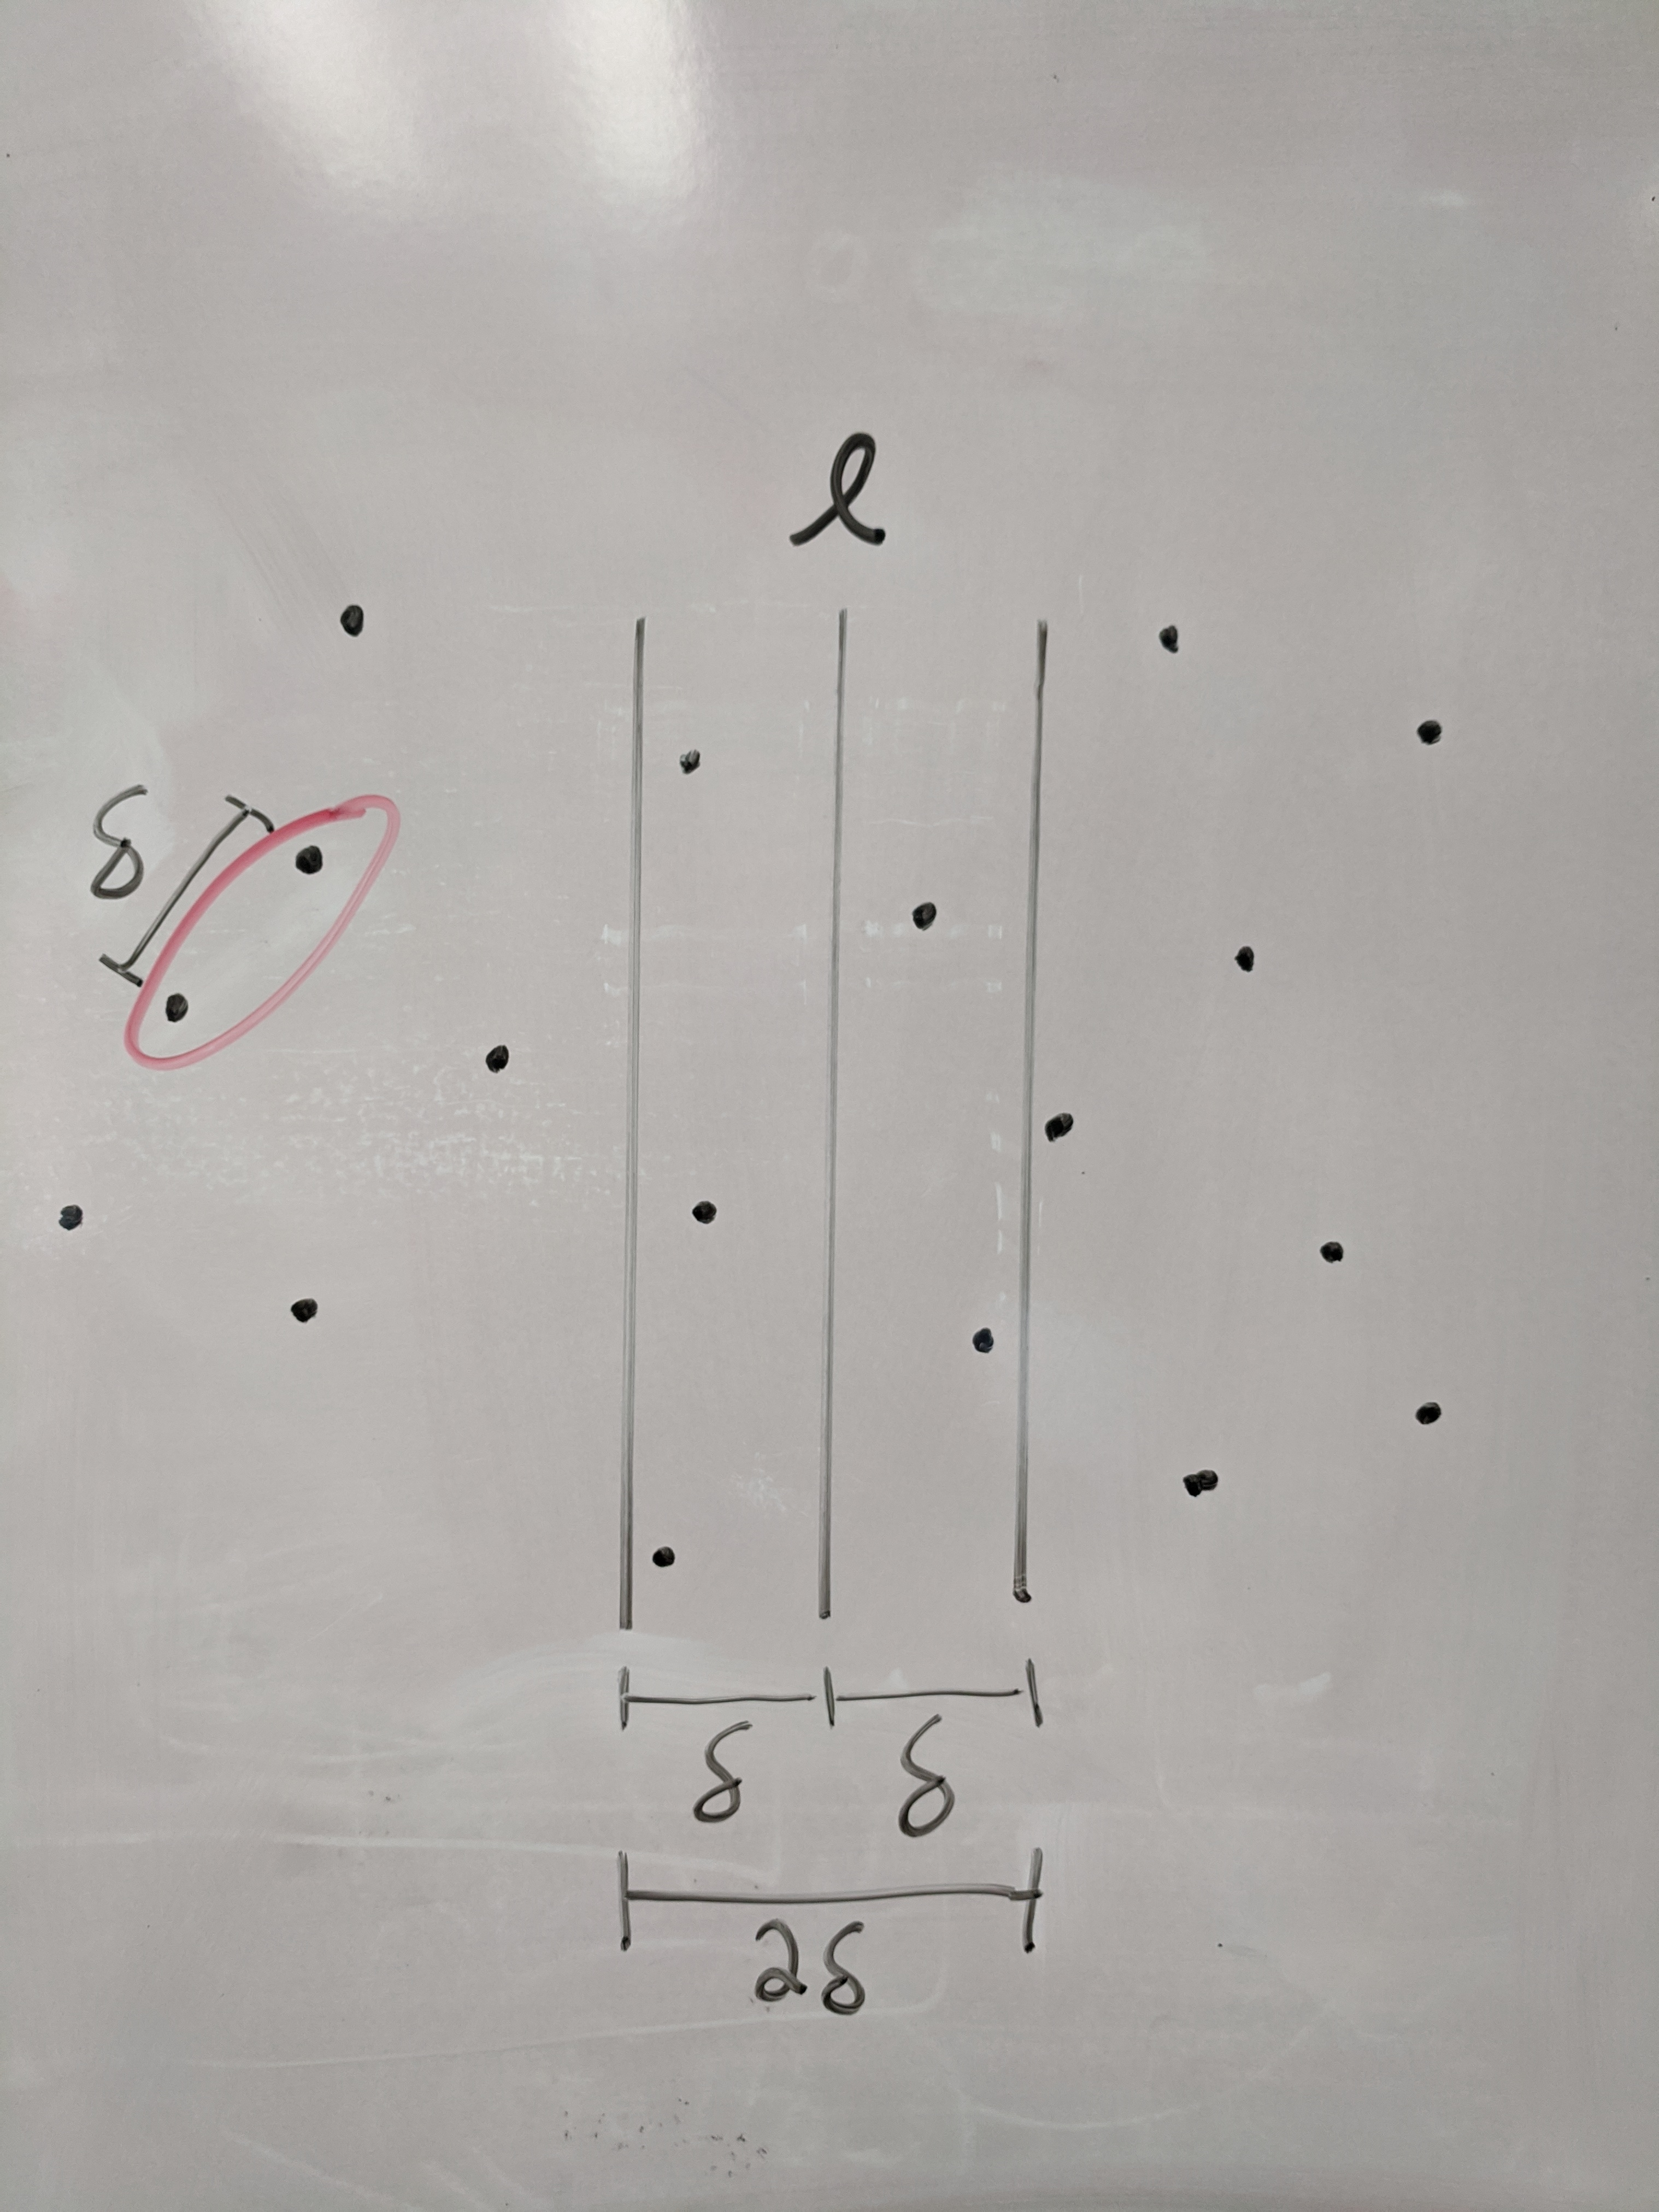
\includegraphics[height=2.5in]{closest-pair-straddling.jpg}
  \end{center}
\end{frame}

\begin{frame} \frametitle{Narrowing Search at Boundary}
\begin{itemize}
  \item \emph{packing argument:} since non-straddling point pairs are separated by $\geq \delta,$
    there are at most 8 non-straddling points in this rectangle (4 per corner of each square)
  \item $\therefore$ for each point $p$ within $\delta$ of $\ell$, test $p$ against
    the 7 points nearest $p$ in $y$-direction
  \item $\leq n$ points within $\delta$ of $\ell$ so $\leq 7n$ pairs of points $\in O(n)$
\end{itemize}
\end{frame}

\begin{frame} \frametitle{Densest Packing of 8 Points all $\delta$ Apart}
  \begin{center}
    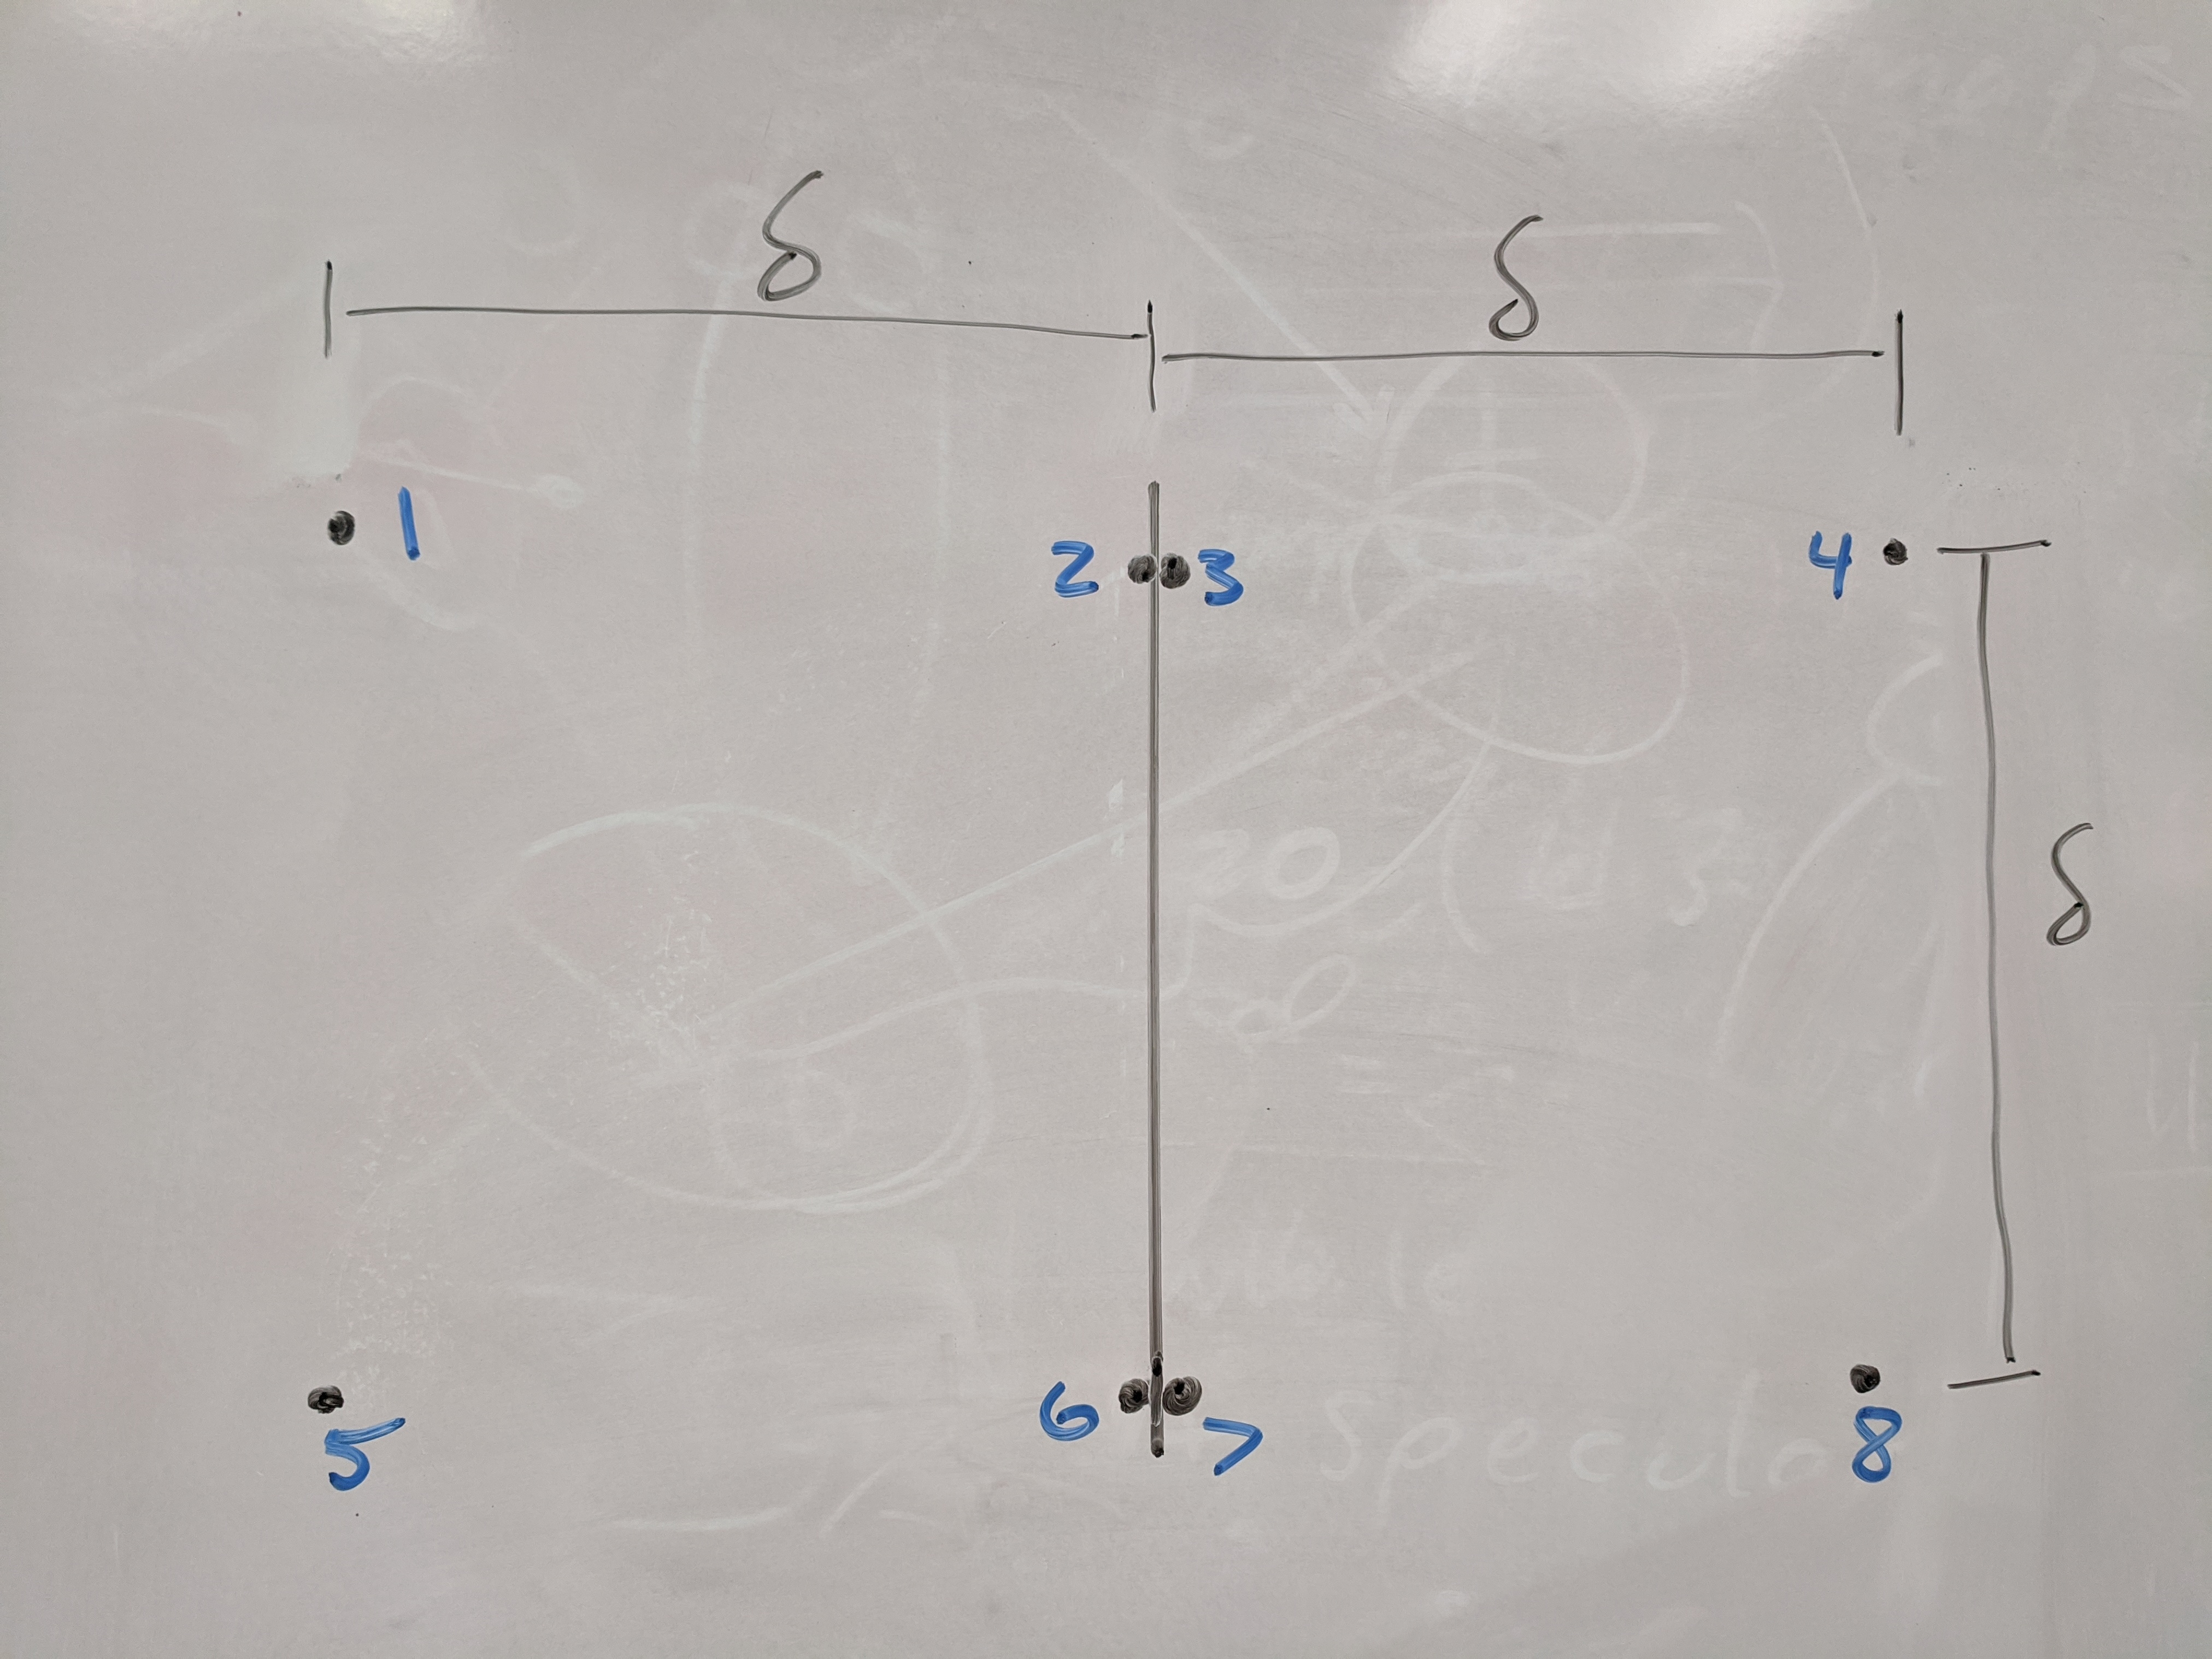
\includegraphics[height=2.5in]{closest-pair-packing.jpg}
  \end{center}
\end{frame}

\begin{frame} \frametitle{Divide-and-Conquer Second Draft}
  {\footnotesize
\begin{algorithmic}[1]
  \Function{CLOSEST-PAIR-DC}{$Q$}
    \If { $n \leq 3$ }
      \State \Return CLOSEST-PAIR-NAIVE($Q$)
    \Else
      \State $X = $ sort $Q$ by $x$-coordinate
      \State $Y = $ sort $Q$ by $y$-coordinate
      \State $\ell$ = vertical line through median $x$-coordinate
      \State $L = \{p \in Q : p \text{ left of } \ell\}, R = Q-L$
      \State $p_L, q_L = $ CLOSEST-PAIR-DC($L$)
      \State $p_R, q_R = $ CLOSEST-PAIR-DC($R$)
      \State $p, q$ = closer of $p_L, q_L$ versus $p_R, q_R$; $\delta=d(p,q)$
      \For { $a \in Q$ and within $\delta$ of $\ell$ }
        \For { 7 points $b$ preceding $a$ in $Y$ }
          \If { $d(a, b) < \delta$ }
            \State $p=a, q=b, \delta=d(a,b)$
          \EndIf
        \EndFor
      \EndFor
      \State \Return $p, q$
    \EndIf
  \EndFunction
\end{algorithmic}
}
\end{frame}

\begin{frame} \frametitle{Second Draft Analysis}
\begin{itemize}
  \item base case is $\Theta(1)$
  \item each sort is $\Theta(n \log n)$
  \item compute $\ell$ is $\Theta(1)$ (given sorted $X$)
  \item build $L, R$ is $\Theta(n)$
  \item straddling \textbf{for} loop is $\Theta(7n) = \Theta(n)$
  \item $T(n) = 2 T(n/2) + \Theta(n \log n)$
  \item by master theorem, $\Theta(n \log^2 n)$
  \item \textbf{bottleneck} is sorting $X, Y$; can do this once before recursion
\end{itemize}
\end{frame}

\begin{frame} \frametitle{Third Draft -- Outer Algorithm}
\begin{algorithmic}[1]
  \Function{CLOSEST-PAIR}{$Q$}
    \State $X = $ sort $Q$ by $x$-coordinate
    \State $Y = $ sort $Q$ by $y$-coordinate
    \State Return CLOSEST-PAIR-HELPER($X$, $X$, $Y$)
  \EndFunction
\end{algorithmic}
\end{frame}

\begin{frame} \frametitle{Third Draft -- Recursive Helper}
  {\footnotesize
\begin{algorithmic}[1]
  \Function{CLOSEST-PAIR-HELPER}{$P$, $X$, $Y$}
    \If { $n \leq 3$ }
      \State \Return CLOSEST-PAIR-NAIVE($P$)
    \Else
      \State $x_m$ = median $x$-coordinate in $P$
      \State $\ell$ = vertical line through $x_m$
      \State $L = \{p \in P : p \text{ left of } \ell\}, R = P-L$
      \State $p_L, q_L = $ CLOSEST-PAIR-HELPER($L$, $X$, $Y$)
      \State $p_R, q_R = $ CLOSEST-PAIR-HELPER($R$, $X$, $Y$)
      \State $p, q$ = closer of $p_L, q_L$ versus $p_R, q_R$; $\delta=d(p,q)$
      \For { $a \in P$ and within $\delta$ of $\ell$ }
        \For { 7 points $b$ preceding $a$ in $Y$ }
          \If { $d(a, b) < \delta$ }
            \State $p=a, q=b, \delta=d(a,b)$
          \EndIf
        \EndFor
      \EndFor
      \State \Return $p, q$
    \EndIf
  \EndFunction
\end{algorithmic}
}
\end{frame}

\begin{frame} \frametitle{Third Draft Analysis}
\begin{itemize}
  \item helper:
    \begin{itemize}
      \item find median $x$ is $\Theta(n)$
      \item (use general median-finding algorithm; or count $k=|P \cap X|$
        then iterate past $k/2$ elements of $X$)
      \item compute $\ell$ is $\Theta(1)$ (given median)
      \item form $L, R$ is $\Theta(n)$
      \item straddling \textbf{for} loop is $\Theta(7n) = \Theta(n)$
      \item $T(n) = 2 T(n/2) + n \in \Theta(n \log n)$ by master theorem
    \end{itemize}
  \item outer algorithm:
    \begin{itemize}
      \item each sort is $\Theta(n \log n)$
      \item helper is $\Theta(n \log n)$
    \end{itemize}
  \item total $\Theta(n \log n)$
\end{itemize}
\end{frame}

\begin{frame} \frametitle{Closest Pair Summary}
Divide-and-conquer algorithm takes $\Theta(n \log n)$ time. \stanza

Builds on
\begin{itemize}
  \item geometric packing argument: checking only $7n$ pairs of straddling points suffices
  \item sort in $\Theta(n \log n)$
  \item median in $\Theta(n)$
  \item master theorem
\end{itemize}
\end{frame}

\end{document}
